%Preamble
\documentclass[12pt,oneside,letterpaper]{article}

% graphicx package, useful for including eps and pdf graphics
\usepackage{graphicx}
\DeclareGraphicsExtensions{.pdf,.png,.jpg}

% basic packages
\usepackage{color}
\usepackage{parskip}
\usepackage{float}

% make links a more pleasing color and don't box them
\definecolor{blue}{rgb}{0.85,0.70,0.99}
\usepackage[hidelinks]{hyperref}
\hypersetup{colorlinks=true,linkcolor=black,citecolor=black,urlcolor=blue}

% text layout
\usepackage{geometry}
\geometry{textwidth=15cm} % 15.25cm for single-space, 16.25cm for double-space
\geometry{textheight=22cm} % 22cm for single-space, 22.5cm for double-space

% helps to keep figures from being orphaned on a page by themselves
\renewcommand{\topfraction}{0.85}
\renewcommand{\textfraction}{0.1}

% bold the 'Figure #' in the caption and separate it with a period
% Captions will be left justified
\usepackage[labelfont=bf,labelsep=period,font=small]{caption}

% review layout with double-spacing
%\usepackage{setspace}
%\doublespacing
%\captionsetup{labelfont=bf,labelsep=period,font=doublespacing}

% cite package, to clean up citations in the main text
\usepackage{cite}

% Remove brackets from numbering in list of References
\renewcommand\refname{\large References}
\makeatletter
\renewcommand{\@biblabel}[1]{\quad#1.}
\makeatother

\usepackage{authblk}
\renewcommand\Authands{ \& }
\renewcommand\Authfont{\normalsize \bf}
\renewcommand\Affilfont{\small \normalfont}
\makeatletter
\renewcommand\AB@affilsepx{, \protect\Affilfont}
\makeatother

% notation
\usepackage{amsmath}
\usepackage{amssymb}

\renewcommand{\vec}[1]{\boldsymbol{#1}}
\newcommand{\Prob}{\mathbb{P}}
\newcommand{\wt}{\text{wt}}
\newcommand{\var}{\text{var}}
\newcommand{\varE}{\text{escape}}
\newcommand{\varT}{\text{transmiss}}
\newcommand{\vac}{\text{vac}}


\title{Transmission mechanisms determine relative fitness and frequency dynamics of viral variants}

\author[1,2,*]{Marlin D.\ Figgins}
\author[1,3]{Trevor Bedford}
\affil[1]{Vaccine and Infectious Disease Division, Fred Hutchinson Cancer Research Center, Seattle, WA, USA}
\affil[2]{Department of Applied Mathematics, University of Washington, Seattle, WA, USA}
\affil[3]{Howard Hughes Medical Institute, Seattle, WA, USA}
\affil[*]{Corresponding author: mfiggins@uw.edu}
\date{\today}
%Figure out author affilations...
% https://maehler.se/blog/2013/11/01/authors-and-affiliations-in-latex

\begin{document}

\maketitle

\begin{abstract}
    Over the course of the COVID-19 pandemic, several SARS-CoV-2 variants have emerged globally, leading to large variant waves in populations of mixed immune backgrounds.
    Classifying these variant viruses into coarse fitness groups has allowed scientists to track the rise and fall of variants by modeling their frequencies over time.
    These models of frequency dynamics enable us to infer fitness advantages in variants, however, these models are typically divorced from a direct interpretation at the level of transmission.
    In this paper, we derive existing frequency dynamic models from exponentially growing populations and extend them to show that relative fitness of variants can be interpreted using compartment models of infectious diseases.
    We use these models to highlight several complications of when analyzing the frequency dynamics for infectious disease variants, namely the difficulty in discovering fitness mechanisms from frequency data alone. 
    We then develop several models for inference of frequency dynamics using Gaussian Processes and dimensionality reduction techniques to estimate latent pseudo-immune components which explain variant dynamics.
    Finally, we apply these models to SARS-CoV-2 sequences in the United States.
     % To better understand the relationship between population dynamics expected from traditional compartment models of epidemics,
\end{abstract}

\section*{Introduction}

The COVID-19 was characterized through large sweeping waves of new variants. 
This phenomenon is consistent with antigenic evolution and is observation in several other viruses such as [INSERT CITATIONS].


To estimate and understand variant turn-over, frequency dynamic models of variant relative fitness have been developed.
These models estimate the relative fitness of circulating variants from frequency data, typically represented by counts of variant sequences over time.
Relative fitness in these models is often assumed to be a constant quantity for simplicity and intrinsic to the variant of interest, however this may not be reasonable due to the nature of the transmission process.

Additionally, translating these relative fitness estimates to a population-level transmission advantage (in terms of variant infections per wildtype infection) requires assumptions on the generation time of the transmission. \cite{Wallinga2006}

%TODO: Mention that we need to make assumptions about transmission process (generation time) to convert to population level

It has been shown that variant transmission advantages differ geographically and temporally which suggests that variant transmission advantages are not necessarily fixed or determined solely due to biology.
Existing models which do allow for variation in variant transmission advantages often do not have a mechanistic underpinning for why these transmission advantages exist and may persist \cite{figgins2022sars, susswein2023leveraging}.
These non-mechanistic transmission advantages are useful for real-time situation analysis though more work must be done to develop theory for how various mechanisms contribute to population change.

We introduce a theory of relative fitness and transmission advantages for exponentially growing populations.
We then apply this to several ordinary differential equation models of epidemics to assess how different transmission mechanisms may contribute to variant turnover and describe relative fitness.
Using these models, we then highlight the importance of population immunity, immune escape, and intrinsic transmissibility in determining variant turnover as well as short term forecasts of frequency growth.

With the knowledge gained from this analysis, we develop several new models of variant frequency dynamics which we use to characterize trade-offs between immune escape and intrinsic transmissibility boosts for pathogens.

%TODO: Throw in generation time change? Then I can discuss work of SWP and mention paper where they showed shorter generation times for Omicron (?)


\section*{Results}

\subsection*{Exponentially growing populations to frequency dynamics}%

We consider a viral population consisting of $V$ exponentially-growing variants with prevalence $I_{v}$ which follows:
\begin{align*}
    \frac{d I_{v}}{d t} = r_{v}(t) I_{v}(t), \quad v = 1,2, \ldots, V.
\end{align*}

Here, $r_{v}(t)$ is the in-homogenous exponential growth rate for variant $v$.

This differential equation has known solution

\begin{align*}
I_{v}(t) = I_{v}(0) \exp\left( \int_{0}^{t} r_{v}(s) ds\right),
\end{align*}
where $I_{v}(0)$ is the initial number of infectious individuals of variant $v$. 

Writing the frequency of variant $v$ in the population as  $f_{v}(t) = I_{v}(t) / \sum_{u=1}^{V} I_{u}(t)$, we can derive an ODE for variant frequency
\begin{align*}
    \frac{d f_{v}}{d t} &= f_{v} \left( \sum_{u=1}^{V} [r_{v}(t) - r_{u}(t)] f_{u} \right)\\
                        &= f_{v} \left( r_{v}(t) - \sum_{u=1}^{V} r_{u}(t) f_{u} \right).
\end{align*}

We can see these equations have the following solution
\begin{align}
    f_{v}(t) &= \frac{ f_{v}(0) \exp( \int_{0}^{t} r_{v}(s) ds)}{\sum_{u=1}^{V}  f_{u}(0) \exp( \int_{0}^{t} r_{u}(s) ds)}
\end{align}


\paragraph{Relative frequency and relative fitness}%

Using the above, we can write the relative frequency of variant $v$ over $u$ as $x_{v,u}(t) = f_{v}(t) / f_{u}(t)$
\begin{align*}
    x_{v, u}(t) = \frac{f_{v}(t)}{f_{u}(t)} &= \frac{f_{v}(0)}{f_{u}(0)} \exp \left( \int_{0}^{t} [r_{v}(s) - r_{u}(s)] ds \right)\\
                                            &=x_{v,u}(0)\exp \left( \int_{0}^{t} \lambda_{v,u}(s) ds \right).
\end{align*}

Notice this relative frequency change depends on the initial relative frequencies and the relative fitness $\lambda_{v,u}(t) = r_{v}(t) - r_{u}(t)$ of $v$ over $u$.
We can notice that this relative frequency is exactly
\begin{align}
\lambda_{v, u}(t) = r_{v}(t) - r_{u}(t) = \frac{d }{d t} \left[\log \left( x_{v,u}(t) \right) \right] = - \lambda_{u,v}(t)
\end{align}

This definition of relative fitness becomes essential in describing various modeling approaches for frequency dynamic data.

\paragraph{Cumulative relative-fitness and frequency change}

From this, we can see that frequency change over time intervals depends only on the cumulative relative fitness over time intervals.
Models of frequency change then can be described in terms of how they represent and estimate these relative fitnesses.
This framework includes various existing methods for analyzing frequency data such as Huddleston et al, MLR, MLR Spline, ...

In the following section, we show this framework applied to several simple compartmental models of epidemics.

\subsection*{Applications to epidemic models}

\paragraph{Two-strain SIR}%

For simplicity, we will begin by analyzing a two-strain SIR based model in which the variant viruses can differ by increased intrinsic transmissibility (via $\eta_{T}$) and immune escape against wild-type immunity (via $\eta_{E}$).
This system of 4 ordinary differential equations is written in full below.

%TODO: Add 3.x
\begin{align*}
    \frac{d S}{d t} &= - \beta S I_{w} - \beta \eta_{T} S I_{v}\\ 
    \frac{d I_{w}}{dt} &= \beta S I_{v} - \gamma I_{w}\\
    \frac{d I_{v}}{dt} &= \beta \eta_{T} S I_{v} + \beta \eta_{T} \eta_{E} \phi_{w} I_{v} - \gamma I_{v}\\
    \frac{d \phi_{w}}{dt} &= - \beta \eta_{T} \eta_{E} \phi_{w} I_{v}
\end{align*}

Writing that $r_{w}(t) = \beta S - \gamma$ and $r_{v}(t) = \eta_{T} \beta  S + \beta \eta_{T} \eta_{E} \phi_{w} - \gamma$, we can then write the relative fitnesses as:
\begin{align*}
\lambda_{v,w}(t) = (\eta_{T} - 1)\beta S(t) + \eta_{T} \eta_{E} \beta \phi_{w}(t).
\end{align*}


We can consider epidemic models which decompose to the form presented in equation (ref).

%TODO: Analysis the tranmissibility-escape trade off by writing out the relative fitness directly.
%TODO: Show that reltive fitness of an emergening immune escape variant depends on the present immunity
%TODO: Additionally that a plane of fitness which depends on the at-risk populations

\paragraph{Models of immune escape against heterogeneous backgrounds}%

We'll now consider a model where all hosts are assumed to fall into one of $B$ immune background $\phi_{b}$ for $b =1, \ldots, B$.
We assume that infection by each variant $v$ then leaves recovered hosts into the corresponding immune background $b_{v}$.
Variant transmission then occurs via immune escape against a background leading to a matrix of escape rates $\vec{\eta} = \eta_{v,b}$ for variants $v$ and background $b$.

We can then write the system of ODEs as 
\begin{align*}
    \frac{d I_{v}}{dt} &= \beta \sum_{1\leq b \leq B} \eta_{v, b} \phi_{b} I_{v} - \gamma I_{v}, \quad v = 1, \ldots, V\\
    \frac{d \phi_{b}}{dt} &= - \beta \sum_{1\leq v \leq V} \eta_{v,b}\phi_{b} I_{v} +  \sum_{v:\ b_{v} = b} \gamma I_{v}
\end{align*}

With this formulation, we can then write the relative fitnesses in terms of the escape rates $\eta_{v,b}$ and the immune background proportions $\phi_{b}$ :

\begin{equation} \label{eq:escape_relative_fitness}
    \lambda_{v, u}(t) = \sum_{1\leq v \leq B}(\eta_{v,b} - \eta_{u,b}) \phi_{b}(t).
\end{equation}

This suggests that the relative fitnesses among variants can be decomposed into differences in immune escape among immune backgrounds within a population.
Understanding the size and complexity of this immune space may therefore be useful for parameterization and forecasting on variant frequencies.

%TODO: Compare this to the model where you explicitly count histories
% These give the same but you are summing over immune histories!

%TODO: Suggest that we might use PCA, SVD, and latent factor models to gain a better understanding of these models

For simplicity, we'll begin with a two variant system with vaccination, so there are three immune background $\phi_{\wt}, \phi_{\var},$ and $\phi_{\vac}$.

(Does this `increase' antigenic evolution? What does that even mean?)

\begin{figure}[h]
    \centering
    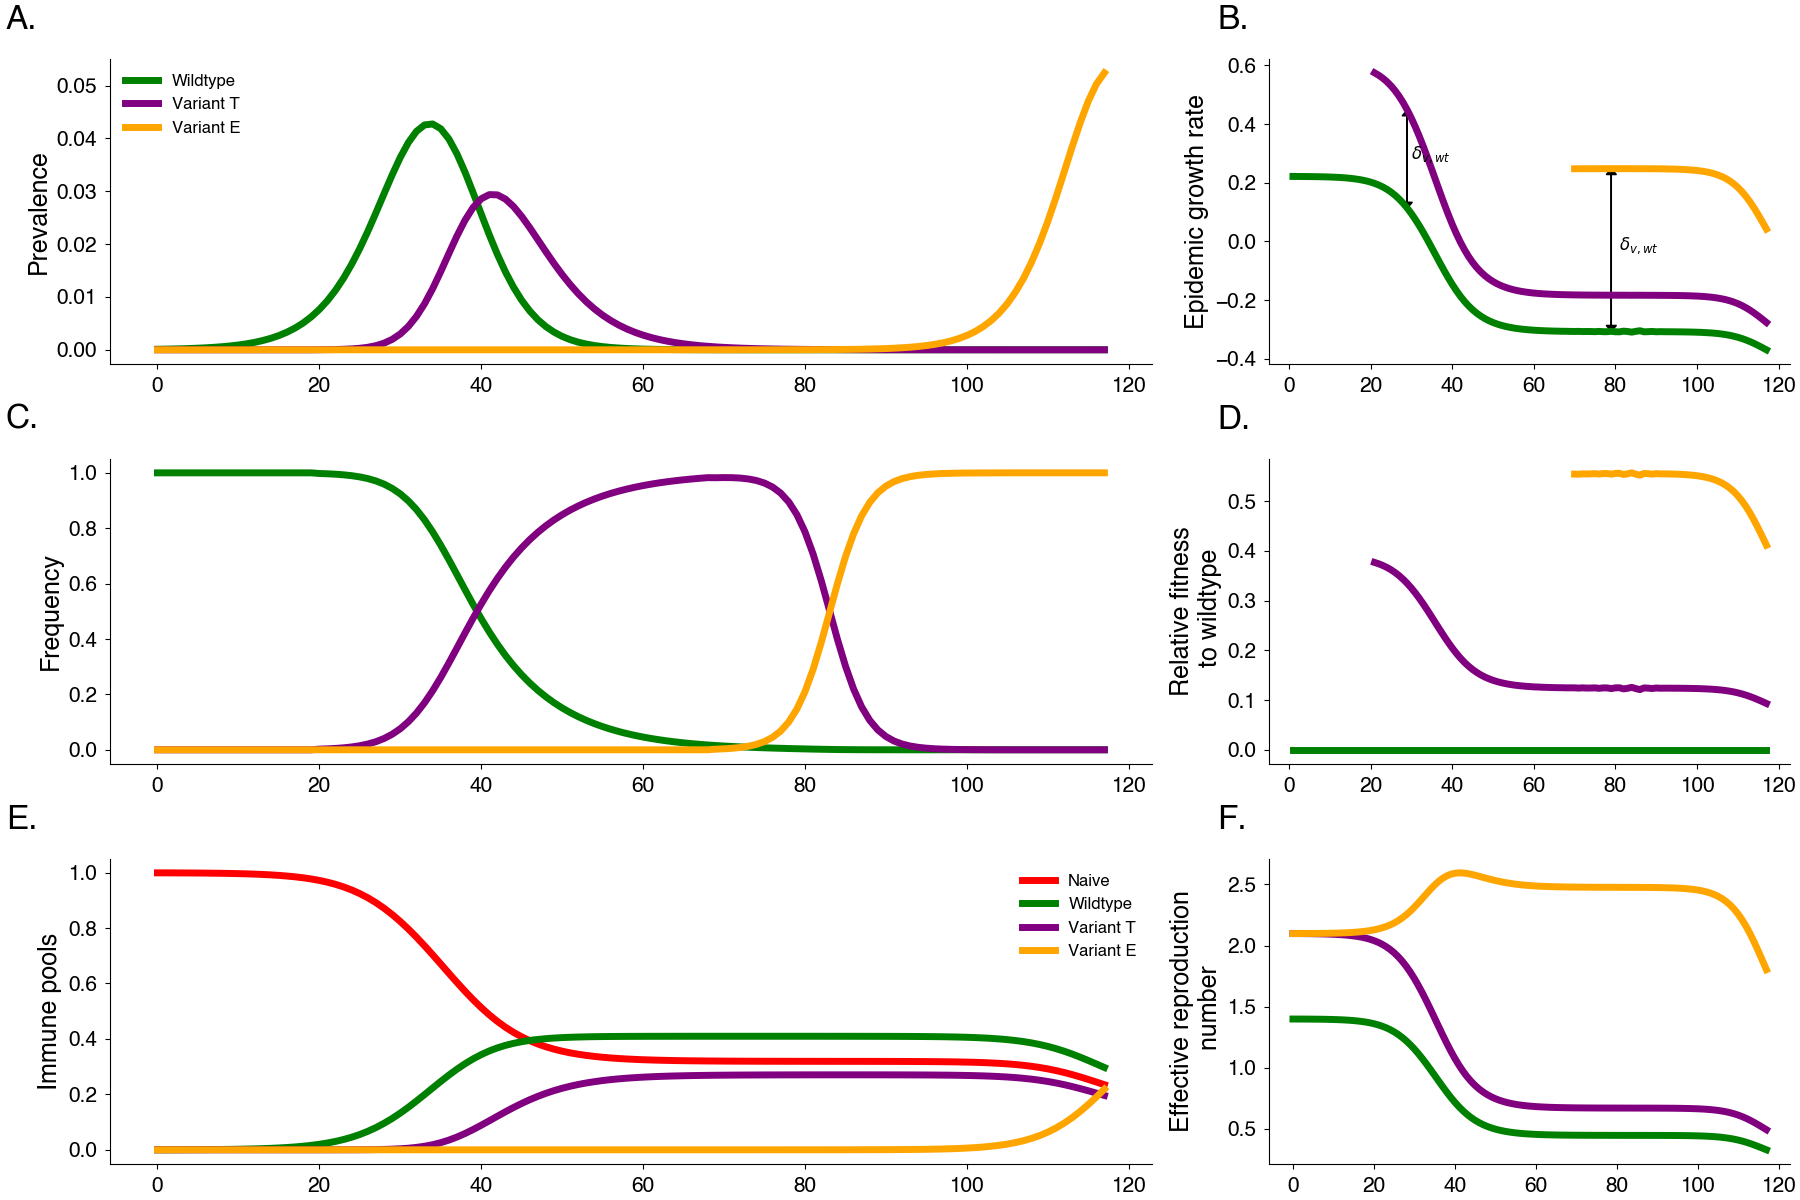
\includegraphics[width=0.8\linewidth]{./figures/vis_mechanisms.png}
    \caption{\textbf{Method overview.} 
    Mechanistic transmission models constrain variant frequency dynamics by specifying a functional form for relative fitnesses.
    Simulations of a three-variant model including a wildtype, one intrinsic transmission increased variant, and one immune escape variant show the relationship between population-level transmission and selection for variants.
    A. Prevalence by variant.
    B. Exponential growth rate by variant.
    C. Variant frequency.
    D. Relative fitness relative to wildtype.
    E. Underlying immune pools.
    F. Effective reproduction number by variant.
}%
    \label{fig:vis_mechanisms}
\end{figure}

\section*{Applications}

Using the theory developed for exponentially-growing variant populations, we now re-visit existing methods for modeling viral frequency dynamics.

\paragraph{Multinomial Logistic Regression}%

We begin with multinomial logistic regression with fixed relative fitnesses (MLR).
This model can be written as

\begin{align*}
    f_{v}(t) = \frac{f_{v}(0) \exp(\lambda_{v} t)}{\sum_{u} f_{u}(0) \exp(\lambda_{u} t)},
\end{align*}

where $f_{v}(t)$ is the frequency of variant $v$ at time $t$ and $\lambda_{v}$ is the relative fitness of variant $v$.
This provides estimates of the relative fitness compared to some reference strain $u^{*}$for which $\lambda_{u^*} = 0$.
Converting this estimate to an estimate of transmission advantage (relative effective reproduction number) requires assuming a delta distribution of the generation time. \cite{Wallinga2006}

We can then see this model results from assuming that the at-risk populations are constant over-time.
This assumption is useful since it requires no outside knowledge of the at-risk population and relative infection rates, though this may be less useful for longer forecasts or when there is large turnover in at-risk populations due to infection.

\paragraph{Flu-forecasting}%

Motivated by the observed antigenic evolution of seasonal influenza, the authors approximate the cumulative relative fitness between flu seasons on the level of individual strains as:

\begin{align*}
    \Lambda_{v,u}(t + \Delta t,t) = \beta_{1} x_{v,1} + \cdots + \beta_{p} x_{v, p} (\Delta t) = \vec{\beta} \cdot \vec{x}_{v} (\Delta t),
\end{align*}

where the relative fitness is determined by strain-specific predictors $\vec{x}_{v}$ and the regression parameter $\vec{\beta}_{v}$ are estimated.
The authors choose predictors which describe the antigenic properties of strains though our previous work in 

\paragraph{Estimating relative fitness using Gaussian Processes}%

We develop a method for using Gaussian processes to model variant relative fitnesses.

%TODO: Provide short explainer on Gaussian processes and use figure from lab meeting as supplemental figure

Here, the relative fitnesses are modeled using a Gaussian process with a ... kernel and shared hyper-parameters.
For efficiency, we implement a Hilbert Space Gaussian Process approximation instead of fitting $V$ independent Gaussian processes since the HSGP allow us to share basis functions \cite{riutortmayol2022practical}.
This model is used in Figure \ref{fig:gp_example} to estimate the relative fitnesses of the simulated variant dynamics in Figure \ref{fig:vis_mechanisms}.

\begin{figure}[h]
    \centering
    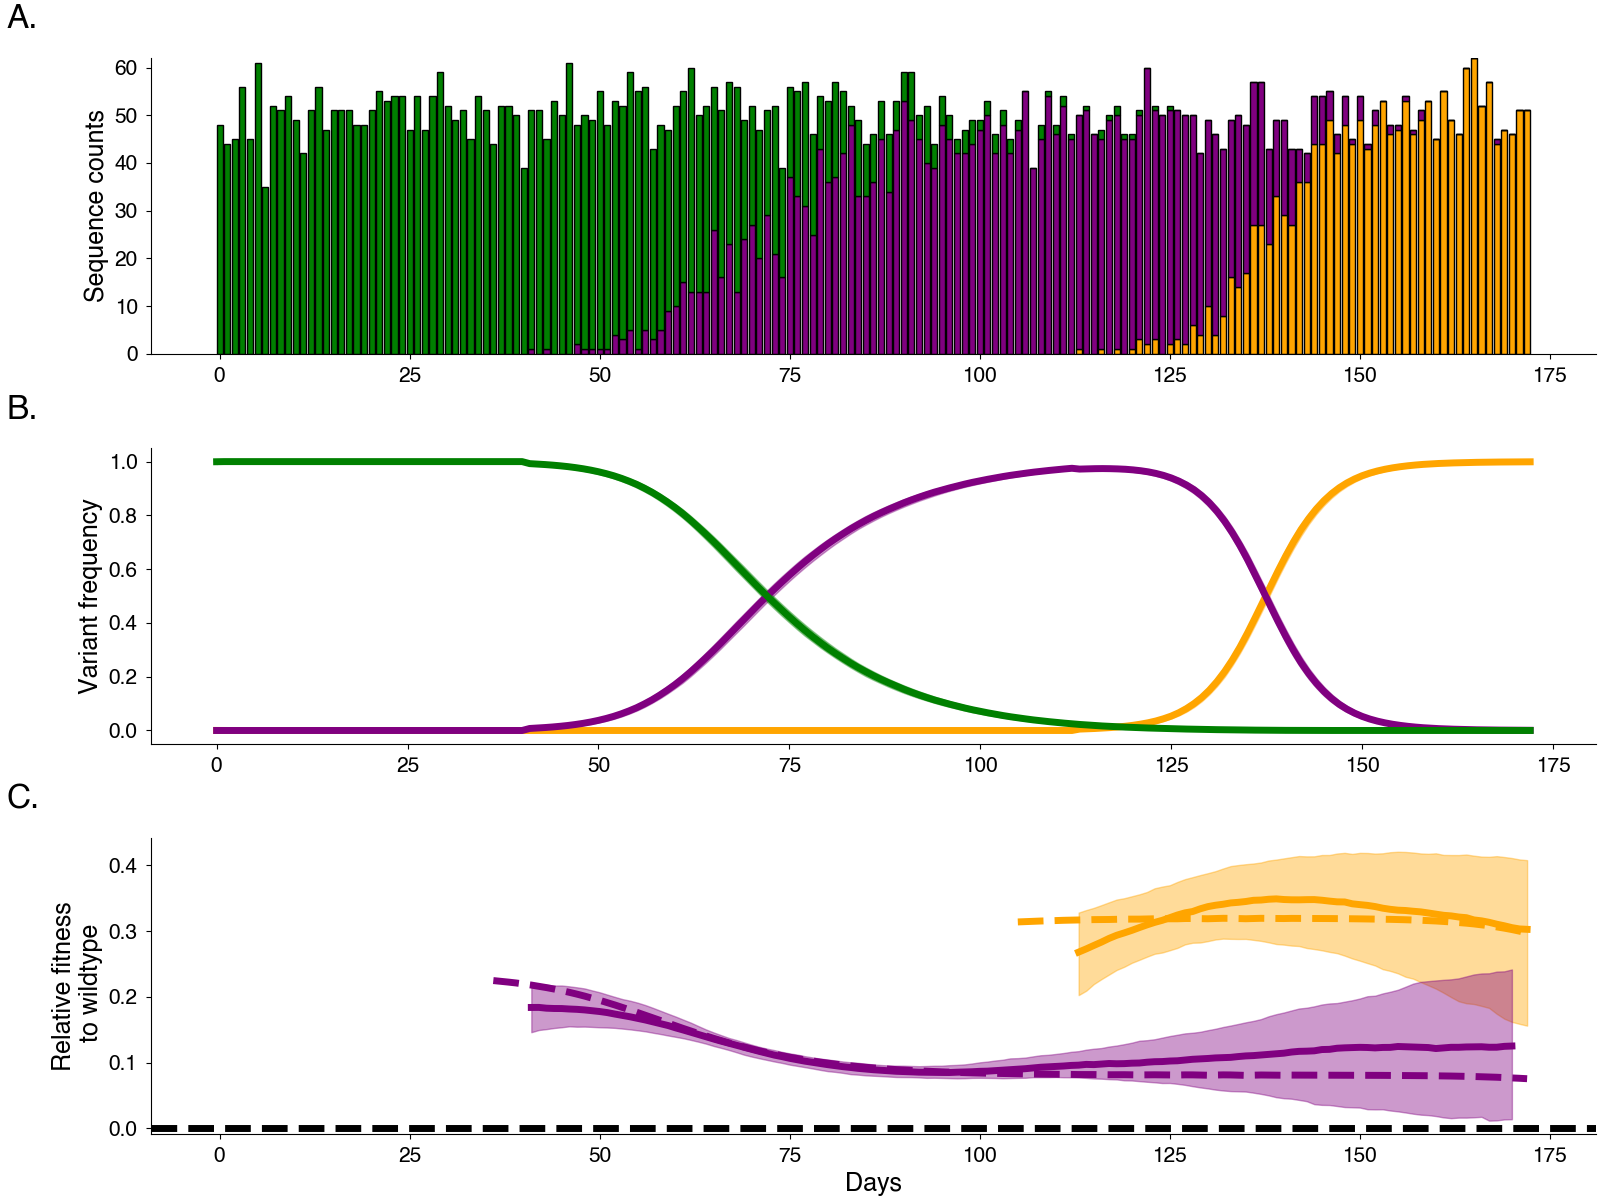
\includegraphics[width=0.8\linewidth]{./figures/gp_example.png}
    \caption{\textbf{Estimating relative fitness with Gaussian Processes.} 
    Gaussian processes allow us a non-parametric estimate of the relative fitness for variants. 
    Below we show an example of using Gaussian processes to model the 3 variant example shown in \ref{fig:vis_mechanisms}.
    A. Sequence counts ...
    B. Frequencies and posterior frequencies according to Gaussian process model. Intervals show the ...\% credible interval.
    C. Relative fitnesses. Dashed line shows true relative fitnesses from mechanistic model. 
}
    \label{fig:gp_example}
\end{figure}


\paragraph{Transmisibility-Escape Tradeoff}%

%TODO: Move this section to tradeoff
Extending this analysis to two variant viruses $v= \wt, \varE, \varT$ such that $\eta_{T}^{\varE} = 1$ and $\eta_{E}^{\varT} = 0$, we can write relative fitnesses an escape only variant or transmissibility increased variant as
\begin{align*}
    \lambda_{\varE, w} &= \eta_{E} \beta \phi_{w}(t)\\
    \lambda_{\varT, w} &= (\eta_{T} - 1) \beta S(t).
\end{align*}

In the simplest case where individuals are either susceptible or have wildtype immunity ($S(t) + \phi_{w}(t) = 1$), we can compute the critical immune fraction $\phi^{*}$ at which $\lambda_{\varE, w}(\phi^{*}) = \lambda_{\varT, w}(\phi^{*})$ as
\begin{equation} \label{eq:critical_immunity}
    \phi^{*} = \frac{\eta_{T} - 1}{\eta_{E} + \eta_{T} - 1}.
\end{equation}

For past exposure level greater than $\phi^{*}$, escape variant have a higher relative fitness.
This trade off shows that increasing escape rate entails that a lower proportion of past exposure is needed for escape variants to be preferred (Figure \ref{fig:transmission_tradeoff}). 
Additionally, this shows that when intrinsic transmissibility increases are limited escape is more likely to be a dominant mechanism for variant turnover.

IDEA: Plot required transmission increase to beat escape variant given initial wave with R0?

IDEA: Shoud I translate this to probability escape variant wins with simple Wright-Fisher simulation?


We visualize this trade-off in Figure \ref{fig:transmission_tradeoff}

\begin{figure}[h]
    \centering
    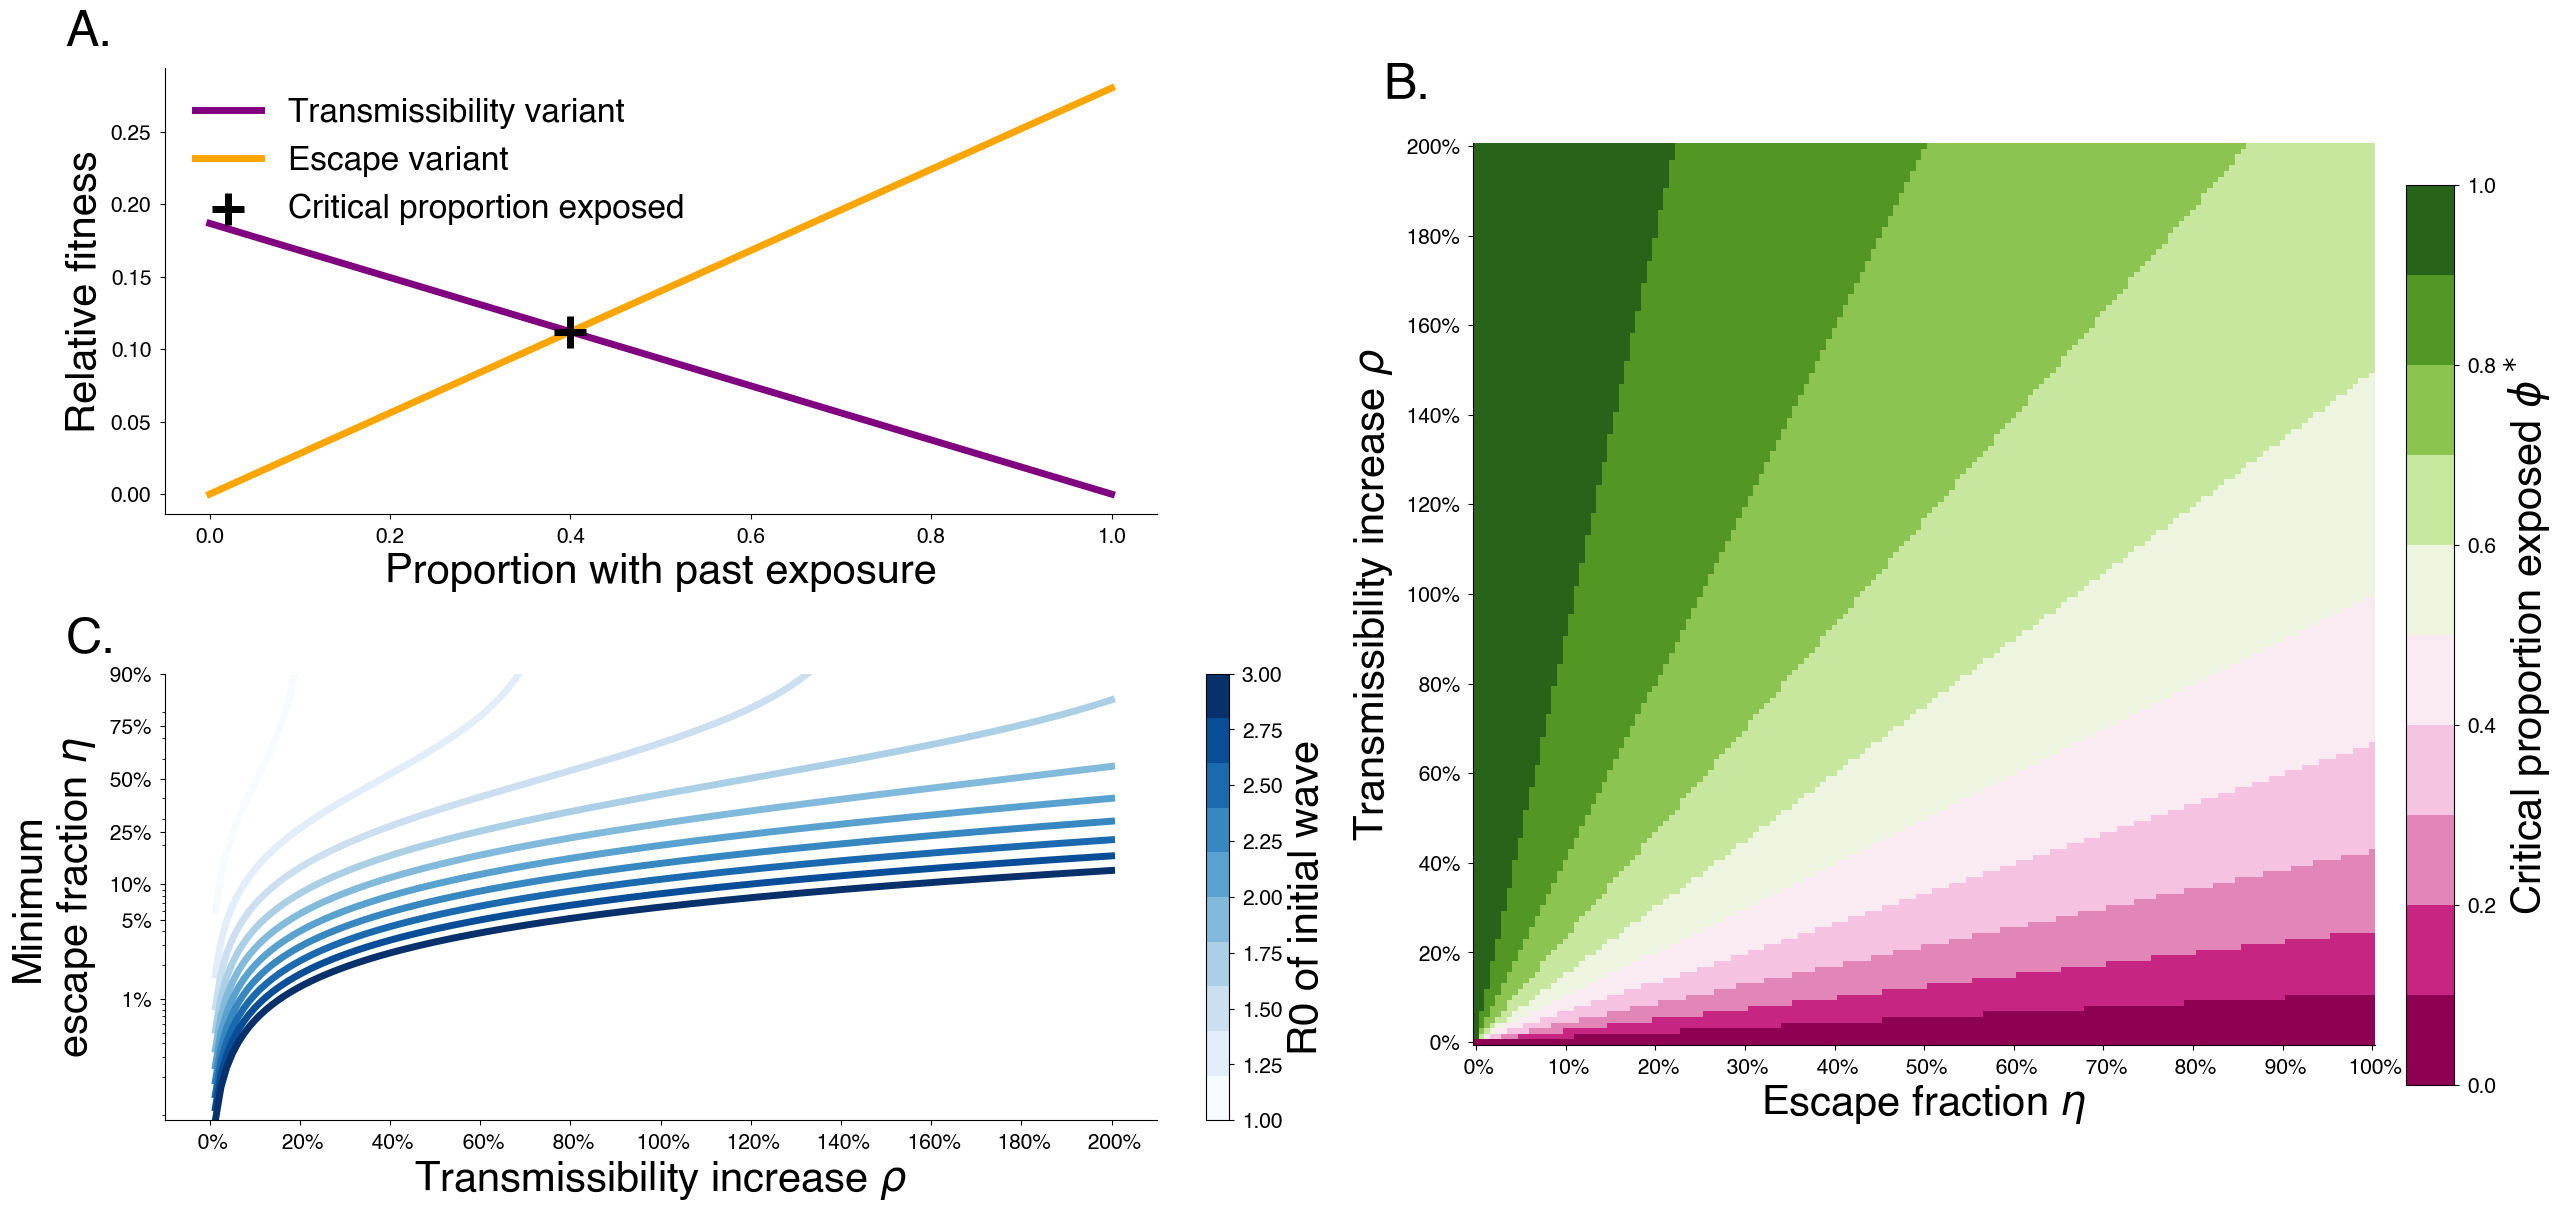
\includegraphics[width=0.8\linewidth]{./figures/transmission_tradeoff.png}
    \caption{\textbf{Trade-off between immune escape and transmissibility increases.} 
    A. Relative fitness for a transmissibility increasing variant and an immune escaping variant for $\eta_{T}=$, $\eta_{E}=$, $\beta=$. 
    The intersection point shows the point after which the escape variant is has higher fitness. 
    B. Modeling escape fraction versus transmissibility increase versus critical proportion exposed for immune escape dominance.}%
    \label{fig:transmission_tradeoff}
\end{figure}

\paragraph{Are initial growth rates sufficient for predicting dominance}%

What happens when there is no mutation? Practical limits given mutation dynamics?
Robustness of relative fitness under similar and varying mechanisms.

\paragraph{How does changing immune pools affect selection?}%
- This is looking at vaccination as a driver of selection

Basically, we want to understand $\lambda(\phi_{1}, \ldots, \phi_{S})$. What do we want to say?

To understand how change in immune-landscape in the host population affects the relative fitness of immune escape variants, we can consider the gradient of an immune escape model

Using equation \ref{eq:escape_relative_fitness}, we can write the gradient of the relative fitness with respect to the immune backgrounds as

\begin{align*}
    \nabla_{\phi} \lambda^{\text{escape}}_{v,u}(t) = (\eta_{v,1} - \eta_{u,1}, \ldots, \eta_{v,B} - \eta_{u,B}).
\end{align*}

From this equation, it's clear that to decrease 


% QUESTION: Can vaccination push you into the regime where escape is preferred? Yes! When is that better overall tho at the population level?
% FIGURE IDEA: For varying vaccination rates, show when escape or transmission is preferred.
% FIGURE IDEA: Show based on simulation with rates probability escape variant wins.

% This probability exists in closed form?

However, decreasing relative fitness for a variant relative to another is not the same as decreasing selection over.
In order to decrease, 

Do we have an idea for variant pressure / total selection here? Can we show whether decreasing selection is same as decreasing cases?

Do we want to consider an expansion in $\frac{d}{d\phi_{s}}$ to assess sensitivity to immune group? What direction increases section overall? (This will come down to just the eta?)
You can have higher selection, but how do cases change in simulation. What would vaccinating against wild-type do? What would vaccinating against variant do? Depends on escape potential against variant?
How does vaccination uptake matter here? Do we want to plot change in relative fitnesses as a function of update? Increased selection but decreased cases

Basically, we want to also monitor decrease in absolute fitness because increased selection pressure =/= increased cases


Is this not the same as the transmissibility trade off? Or are we considering two immune escaping?
We want to think explicitly about vaccination and selection for variants?
Could we treat this similar to SWP leaky paper where some fraction is reset or leaky vaccine to see what changes depending on vaccine efficacy
Basically, vaccination can push you into the zone where escape is preferred :O (SEE ABOVE)

\paragraph{Correlations are insufficient for mechanism identification}%

\paragraph{Predictive capabilities of simple models on complex dynamics}%

\paragraph{Dimensionality of immune space}%

\paragraph{Latent factor models of relative fitness}

\ref{fig:latent_immune}
%TODO: Extend this section to use more recent data, embed pango lineages?

\begin{figure}[h]
    \centering
    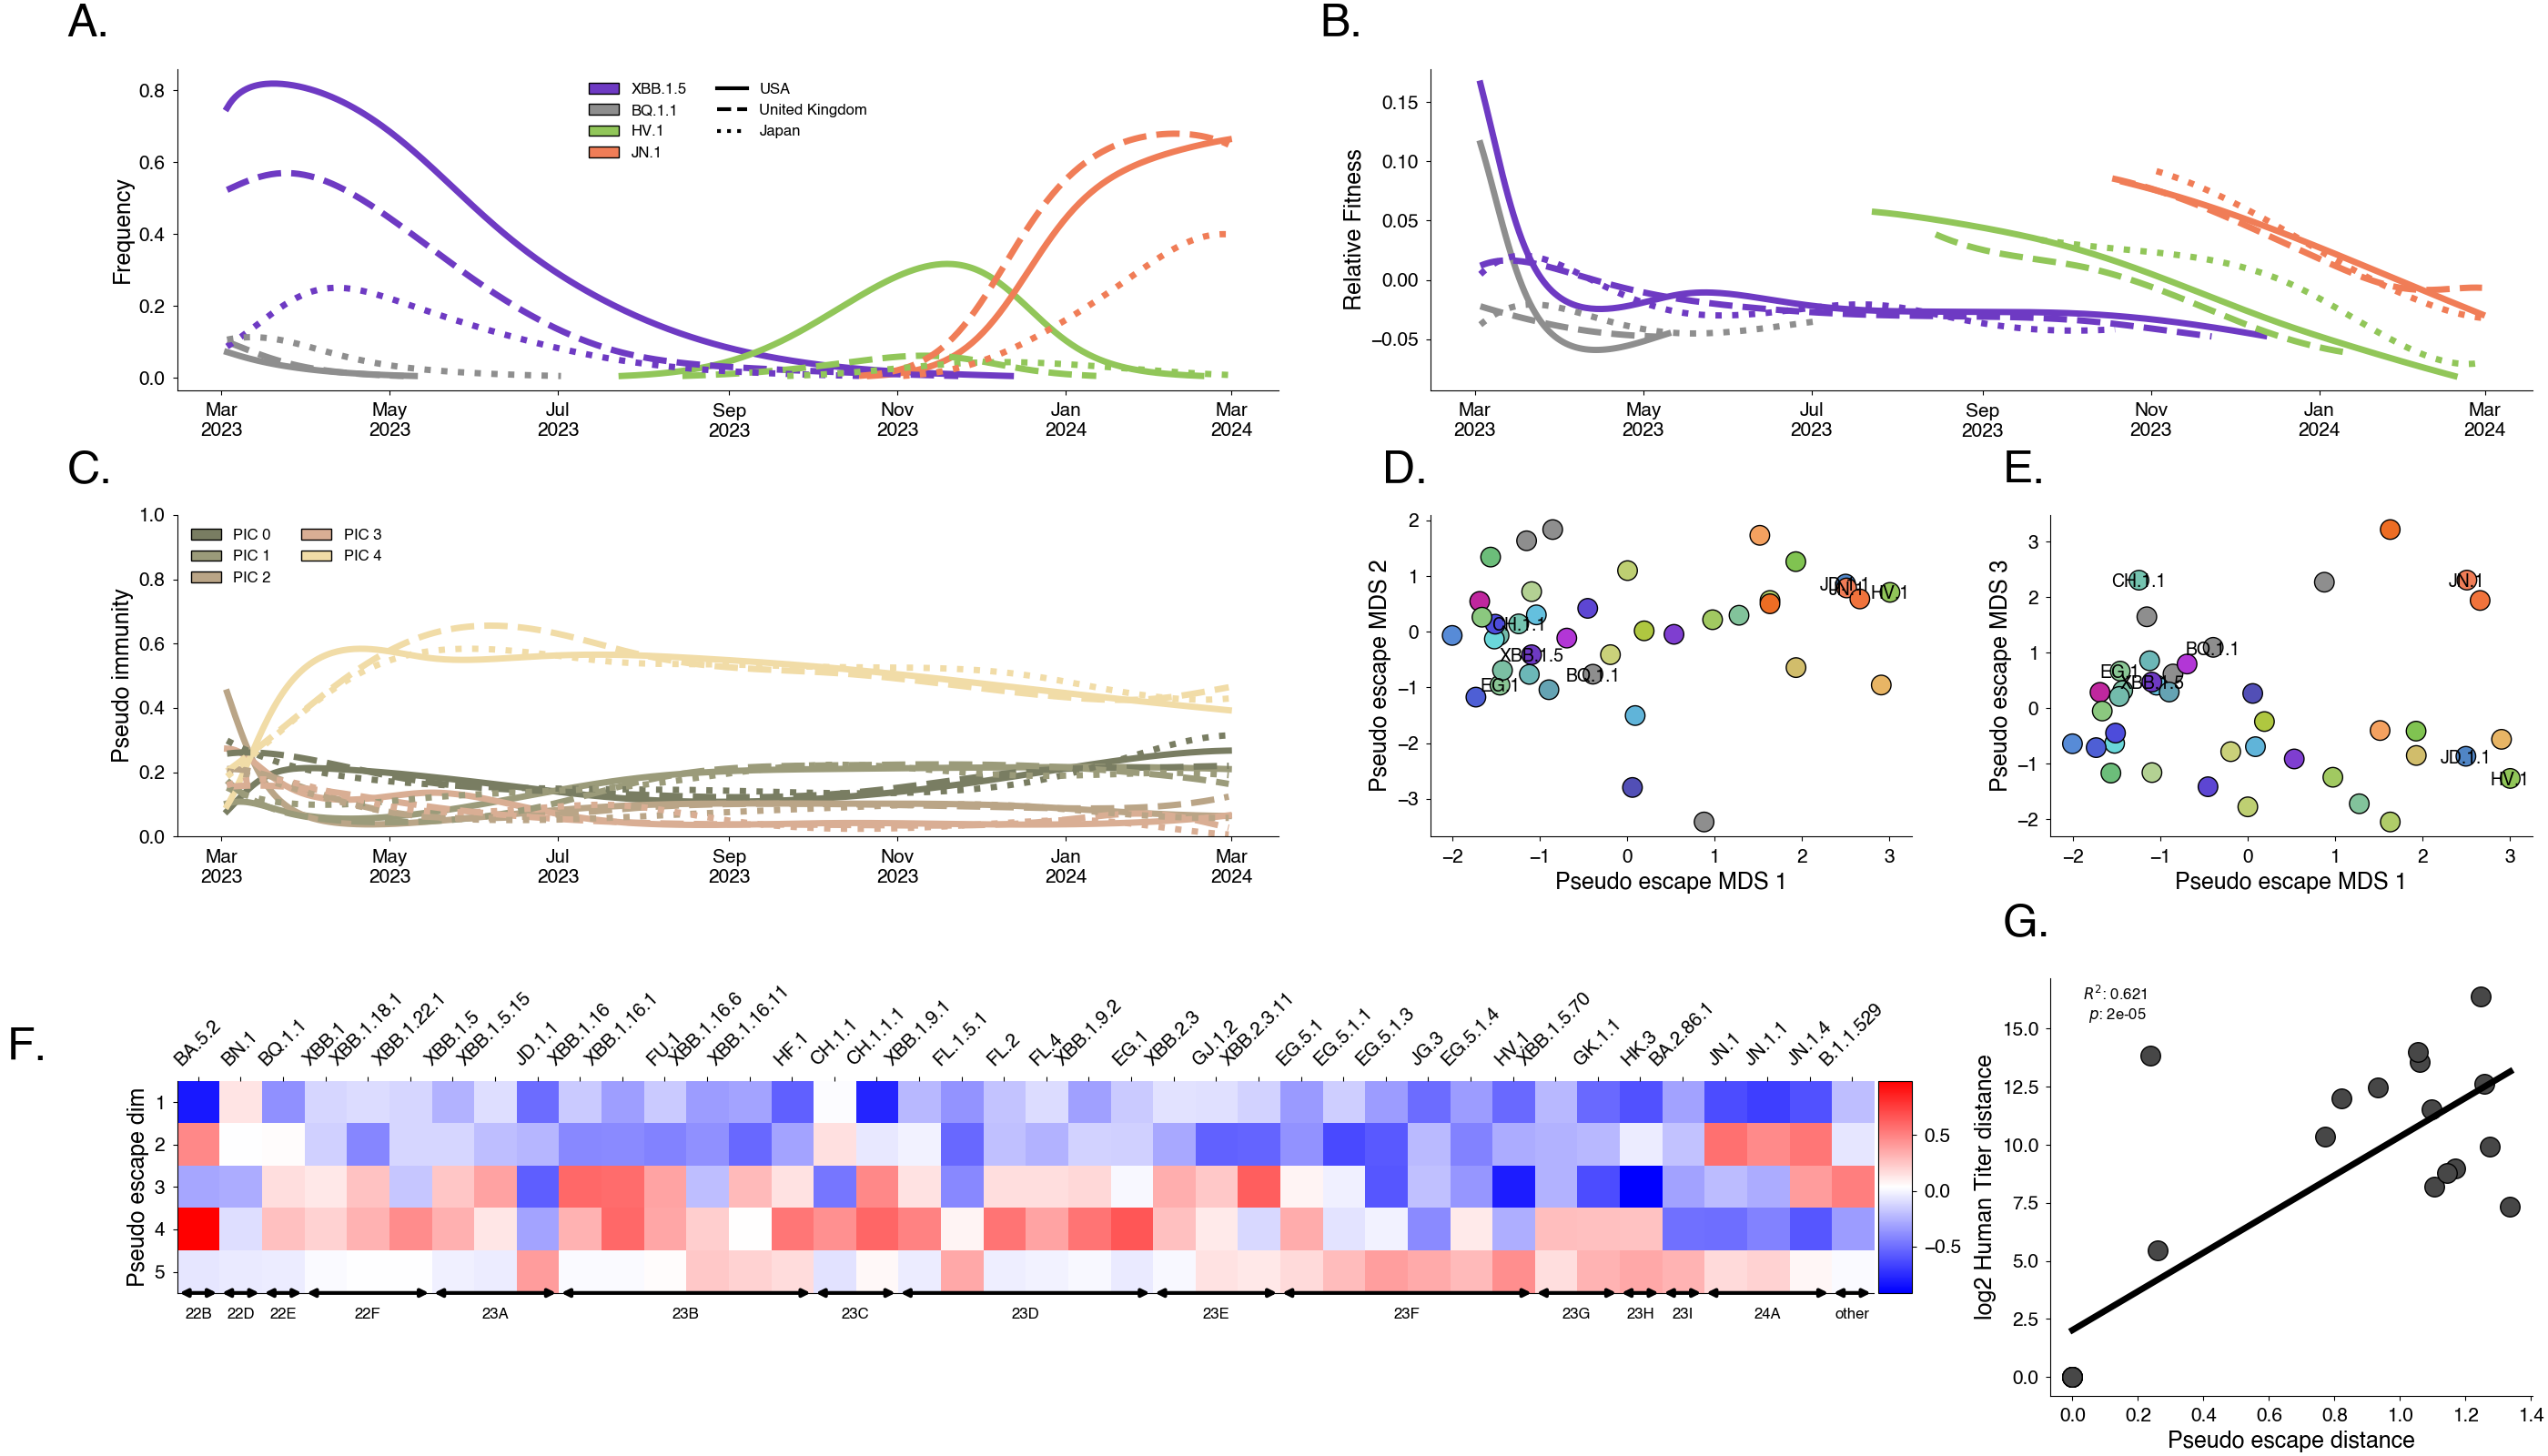
\includegraphics[width=0.8\linewidth]{./figures/latent_immune.png}
    \caption{\textbf{Latent factor models of immunity describe variant structure.} 
        We fit the latent immunity factor model to early SARS-CoV-2 frequency data.
        A. Variant frequency. Points are the sample frequencies and the thick lines are modeled variant frequencies. Each is colored by variant of concern.
        B. Estimated relative fitness for each variant.
        C. Estimated pseudo-immunity over time.
        D. Estimated pseudo-escape rates for each variant.
        E. Dimensionality-reduced pseudo-escape rates using Multidimensional Scaling.
    }
    \label{fig:latent_immune}
\end{figure}


%TODO: Could be useful to directly compare to published antigenic cartography work as mentioned before ...

\section*{Discussion}

Mention limitations of generation time assumptions for compartmental epidemic models

%TODO: Discuss extensions to Laplace transform method
% We can 1.8 from my general exam to compute roots
% We can then compute fitness
Limitations of deterministic fitness models 


\section*{Methods}

\paragraph{Generating sequence counts}%

\cite{aksamentov2021nextclade}
\cite{Hadfield2018}

\paragraph{Likelihood of sequence counts given frequencies}

The models discussed in this paper use counts of variant sequences to inform the underlying variant frequency in the population.
This is accomplished using a multinomial likelihood, so that given counts of sequences $C_{t,v}$ of variant $v$ at time $t$ and total sequences $N_{t}$ collected at time $t$, we have that

\begin{equation*}
    C_{t, \cdot} \sim \text{Multinomial}(N_{t}, f_{v}(t)),
\end{equation*}

where $f_{v}(t)$ is the frequency of variant $v$ at time $t$.
This is a simple model of sequence counts to frequencies and does not account for over-dispersion of sequence counts relative to a multinomial, however, all models can be extended to estimate and account for over-dispersion by replacing the above likelihood with a Dirichlet-Multinomial likelihood.

\paragraph{Gaussian process model}%

To generate smooth non-parametric estimates of variant growth rates, we develop a Gaussian process based model for relative fitnesses. 
That is, we model the relative fitness for each variant $v$ over time as a multivariate normal distribution

\begin{align*}
    \vec{\lambda}_{v} &\sim \text{Normal}(\vec{\mu}, \vec{\Sigma})\\
    \vec{\Sigma}_{s, t} &= K_{\theta}(s, t),
\end{align*}
where $K_{\theta}$ is a potentially parameterized kernel function. 
This induces a structure on the covariance of the relative fitness values over time.

For computational efficiency, we implement a Hilbert Space Gaussian process approximation, so that the relative fitnesses can be represented linearly as

\begin{equation}
    \lambda_{v}(t) \approx \sum_{j=1}^{m} S_{\theta}(\sqrt{\mu_{j}})^{1/2} \cdot \phi_{j}(x) \cdot \beta_{j},
\end{equation}
where $S_{\theta}$ is the spectral density of the kernel $K$, $\mu_{j}$ and $\phi_{j}$ are the eigenvalues and eigenfunctions of the Laplacian, and $\beta_{j} \sim \text{Normal}(0,1)$ \cite{riutortmayol2022practical}.
Since the eigenvalues and eigenfunctions are shared across variants, this allows us to re-use values across variants, simplifying the computation to a matrix multiplication as

%TODO: Fix this
\begin{equation*}
    \vec{\lambda}_{t,v} = \vec{\Phi}\vec{S}_{\theta}\vec{\beta}.
\end{equation*}


\paragraph{Latent immune factor model}%

We show that relative fitnesses dynamics ought to be explained by low-dimensional immunity when transmission dynamics are described with compartment models.
This motivated a model to learn this low-dimensional structure that is inspired by latent-factor models. We start by assuming that the relative fitness of variant $v$ at time $t$ and in geographic location $g$ can be described by $D$ latent factors so that

\begin{equation}
    \lambda_{v}^{g}(t) = \sum_{d=1}^{D} \eta_{v,d} \phi_{d}^{g}(t). 
\end{equation}
As the structure here resembles Equation \ref{eq:escape_relative_fitness}, we call the $\eta$ ``pseudo-escape'' and $\phi_{d}^{g}$ the ``pseudo-immunity''.
To make this more consistent with our intuition here, we model $\phi_{d}^{g}$ to be in $[0,1]$ and model it as smoothly varying in time.
In the results shown above, we model $\text{logit}(\phi_{d}^{g})$ using splines.
Additionally, in order to prevent degeneracies in the parameter estimates, we fix some base variant $v^*$ which fitness is defined relative to, so that $\eta_{v^*, d} = 0$ for all $1\leq d\leq D$.
We also order the components in the first geography for identifiability.


\subsection*{Data and code accessibility}

Source code used to generate figures are available at. 
Additionally, implementations of all models discussed are included at ...

\subsection*{Competing interests}%

\subsection*{Author contributions}
MF conceived the study. 
% TB gathered sequence and case count data. 
MF designed and implemented inference models. 
MF performed the analysis. 
% MF, TB interpreted the results. 
% MF, TB wrote the paper.


\subsection*{Acknowledgements}%

\bibliographystyle{plos}
\bibliography{relative-fitness-mechanisms}

\newpage

\appendix

\setcounter{figure}{0}
\setcounter{table}{0}
\setcounter{page}{1}
\renewcommand{\thefigure}{S\arabic{figure}}
\renewcommand{\thetable}{S\arabic{table}}
\renewcommand{\thepage}{S\arabic{page}}

\section*{Supplemental Appendix}

\subsection*{Relative fitness for full immune history models}%

%TODO: Define sets then you simplified
$\mathcal{P}(M \setminus \{i\})$

We show that the simple background model is consistent with an expanded immune history model. 
Beginning with the model from Lazebnik and Bunimovich-Mendrazitsky 2022 \cite{Lazebnik2022}, we consider the differential equation for the individuals with strain infection history $J$ and current infecting strain $i$ $R_{J}I_{i}$
\begin{align*}
\frac{dR_{J} I_{i}}{dt} = - \gamma_{J, i} R_{J} I_{i} + \beta_{J, i} R_{J} \sum_{K \in P(M), i\notin K} R_{K}I_{i}.
\end{align*}

Here, infection can occur from any individual infected with strain $i$ assuming their past immune history does not include $i$ and the infected are any recovered individual with immune history $J$  $R_{J}$.
To compute the strain growth rate, we can sum over all possible immune histories for individuals infected with strain $i$, so that
\begin{align*}
    \frac{d I_{i}}{d t} &= \sum_{J \in P(M), i \notin J} \frac{dR_{J} I_{i}}{dt} \\
                        &= - \gamma_{i} I_{i} + \sum_{J \in P(M), i \notin J} \beta_{i, J} R_{J} \sum_{K \in P(M), i\notin K} R_{K}I_{i}\\
                        &= - \gamma_{i} I_{i} + \sum_{J \in P(M), i \notin J} \beta_{i, J} R_{J} I_{i}\\
                        &= \left(-\gamma_{i} + \sum_{J \in P(M), i \notin J} \beta_{i,J} R_{J} \right) I_{i}\\
                        &= \left(-\gamma + \beta\sum_{J \in P(M), i \notin J} \eta_{i,J} R_{J} \right) I_{i}\\
\end{align*}

Assuming that the transmission rate can be decomposed as a base transmission rate $\beta$ and a strain $i$ and immune history $J$ specific escape rate $\eta_{i, J}$ and that the recovery rate is constant, we notice this is identical to our previous immune background model.
Therefore, our relative fitnesses can be written as

\begin{align*}
    \lambda_{i, j} = \sum_{B \in P(M)} (\eta_{i, B} - \eta_{j, B}) R_{B},
\end{align*}
where for simplicity we define $\eta_{v, B} = 0$ if $v \in B$.


\end{document}
